
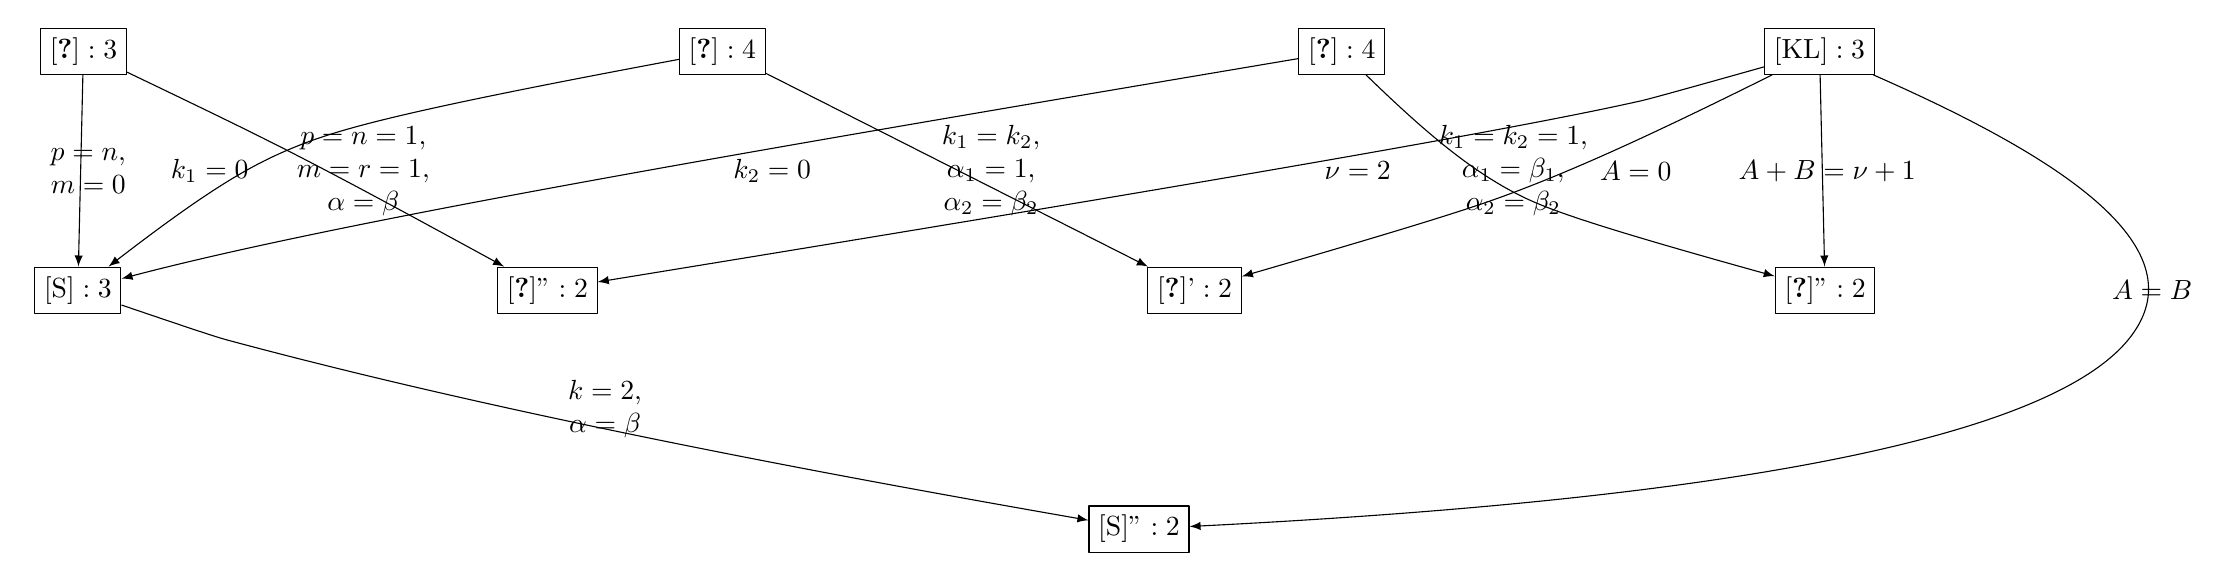
\begin{tikzpicture}[>=latex,line join=bevel,]
%%
\node (DF85) at (103.87bp,190.0bp) [draw,rectangle] {$\mbox{\cite{dotsenko1985four}}:3$};
  \node (Spp) at (483.87bp,18.0bp) [draw,rectangle] {$\mbox{[S]''}:2$};
  \node (KL) at (728.87bp,190.0bp) [draw,rectangle] {${\mbox{[KL]}}:3$};
  \node (S) at (101.87bp,104.0bp) [draw,rectangle] {$\mbox{[S]}:3$};
  \node (War10) at (556.87bp,190.0bp) [draw,rectangle] {$\mbox{\cite{warnaar2010sl3}}:4$};
  \node (TV03p) at (503.87bp,104.0bp) [draw,rectangle] {$\mbox{\cite{tarasov2003selberg}'}:2$};
  \node (DF85pp) at (270.87bp,104.0bp) [draw,rectangle] {$\mbox{\cite{dotsenko1985four}''}:2$};
  \node (TV03) at (333.87bp,190.0bp) [draw,rectangle] {$\mbox{\cite{tarasov2003selberg}}:4$};
  \node (War10pp) at (730.87bp,104.0bp) [draw,rectangle] {$\mbox{\cite{warnaar2010sl3}''}:2$};
  \draw [->] (DF85) ..controls (153.32bp,166.32bp) and (166.17bp,159.99bp)  .. (177.87bp,154.0bp) .. controls (194.65bp,145.41bp) and (212.95bp,135.66bp)  .. (DF85pp);
  \definecolor{strokecol}{rgb}{0.0,0.0,0.0};
  \pgfsetstrokecolor{strokecol}
  \draw (204.62bp,147.0bp) node {$\begin{array}[]{c}p=n=1,\\m=r=1,\\\alpha=\beta\end{array}$};
  \draw [->] (TV03) ..controls (211.78bp,167.2bp) and (193.24bp,161.29bp)  .. (176.37bp,154.0bp) .. controls (160.89bp,147.31bp) and (145.17bp,137.33bp)  .. (S);
  \draw (177.62bp,147.0bp) node {$\kern-2cm k_1=0$};
  \draw [->] (KL) ..controls (669.18bp,173.22bp) and (666.5bp,172.59bp)  .. (663.87bp,172.0bp) .. controls (612.57bp,160.49bp) and (483.81bp,138.7bp)  .. (DF85pp);
  \draw (562.62bp,147.0bp) node {$\nu=2$};
  \draw [->] (TV03) ..controls (395.58bp,158.78bp) and (431.12bp,140.8bp)  .. (TV03p);
  \draw (430.62bp,147.0bp) node {$\begin{array}[]{c}k_1=k_2,\\ \alpha_1=1,\\\alpha_2=\beta_2\end{array}$};
  \draw [->] (KL) ..controls (729.56bp,160.36bp) and (729.91bp,145.43bp)  .. (War10pp);
  \draw (731.62bp,147.0bp) node {$A+B=\nu+1$};
  \draw [->] (War10) ..controls (586.22bp,161.43bp) and (601.7bp,148.54bp)  .. (617.37bp,140.0bp) .. controls (627.58bp,134.44bp) and (638.78bp,129.58bp)  .. (War10pp);
  \draw (618.62bp,147.0bp) node {$\begin{array}[]{c}k_1=k_2=1,\\\alpha_1=\beta_1,\\\alpha_2=\beta_2\end{array}$};
  \draw [->] (DF85) ..controls (103.18bp,160.36bp) and (102.83bp,145.43bp)  .. (S);
  \draw (105.62bp,147.0bp) node {$\begin{array}[]{c}p=n,\\m=0\end{array}$};
  \draw [->] (KL) ..controls (814.8bp,152.26bp) and (867.3bp,119.17bp)  .. (839.87bp,86.0bp) .. controls (802.66bp,41.004bp) and (632.28bp,25.51bp)  .. (Spp);
  \draw (848.62bp,104.0bp) node {$A=B$};
  \draw [->] (S) ..controls (149.68bp,87.72bp) and (152.82bp,86.822bp)  .. (155.87bp,86.0bp) .. controls (249.55bp,60.769bp) and (360.42bp,39.545bp)  .. (Spp);
  \draw (291.62bp,61.0bp) node {$\begin{array}[]{c}k=2,\\\alpha=\beta\end{array}$};
  \draw [->] (War10) ..controls (354.52bp,155.87bp) and (198.64bp,129.53bp)  .. (S);
  \draw (351.82bp,147.0bp) node {$k_2=0$};
  \draw [->] (KL) ..controls (672.14bp,161.77bp) and (645.37bp,149.39bp)  .. (620.87bp,140.0bp) .. controls (607.17bp,134.75bp) and (592.34bp,129.71bp)  .. (TV03p);
  \draw (655.62bp,147.0bp) node {$\kern0.5cm A=0$};
%
\end{tikzpicture}
